\documentclass[12pt,epsf]{report}
\usepackage[left=2cm, right=2cm, bottom=2cm,top=2cm]{geometry}
\usepackage[myheadings]{fullpage}
\usepackage{fancyhdr}
\usepackage{lastpage}
\usepackage{graphicx, wrapfig, subcaption, setspace, booktabs}
\usepackage[T1]{fontenc}
\usepackage[font=small, labelfont=bf]{caption}
\usepackage{fourier}
\usepackage[protrusion=true, expansion=true]{microtype}
\usepackage[english]{babel}
\usepackage{sectsty}


\newcommand{\HRule}[1]{\rule{\linewidth}{#1}}
\onehalfspacing
\setcounter{tocdepth}{5}
\setcounter{secnumdepth}{5}

%-------------------------------------------------------------------------------
% HEADER & FOOTER
%-------------------------------------------------------------------------------
\pagestyle{fancy}
\fancyhf{}
\setlength\headheight{15pt}
\fancyhead[L]{Group Number 6}
\fancyhead[R]{Statistical Methods in Research}
\fancyfoot[R]{Page \thepage\ of \pageref{LastPage}}
%-------------------------------------------------------------------------------
% TITLE PAGE
%-------------------------------------------------------------------------------

\begin{document}

\title{ \large \textsc{Statistical Methods in Research}
		\\ [2.0cm]
		\HRule{1pt} \\
		\LARGE \textbf{{Analysis of How Stress Patterns Define Human Experience and Performance in Dexterous Tasks}}
		\HRule{1pt} \\ [0.5cm]
		\normalsize \today \vspace*{5\baselineskip}}

\date{}

\author{
		Suchismitha Vedala \\ 
		Lavanya Rao \\
		Yashwanth Reddy Venati }

\maketitle
\tableofcontents
\newpage

%-------------------------------------------------------------------------------
% Section title formatting
\sectionfont{\scshape}
%-------------------------------------------------------------------------------

%-------------------------------------------------------------------------------
% BODY
%-------------------------------------------------------------------------------

\section*{Introduction}
\addcontentsline{toc}{section}{Introduction}
{The Microsurgery performance data represents the performance of 22 medical students in microsurgery activities. The 22 medical students or subjects in our analysis, participated in a longitudinal study regarding the relationship of sympathetic arousal and skill in learning micro-surgical tasks. The subjects had to pay five visits which we regard as sessions, lasting one hour each, in order to practice micro-surgical cutting and suturing in an inanimate simulator.A pre and post study questionnaire was also given to be completed by the subjects to know a little about their biography and anxiety.\\
\\
During the main part of each session, the subjects underwent the following treatments:\\
1.Baseline: The subjects were relaxing for 5 min, listening to spa music. They were facially recorded by a thermal and visual camera.\\
2.Cutting: The subjects had to precision cutting in the inanimate simulator. They were facially recorded by a thermal and visual camera.\\
3.Suturing: The subjects had to perform suturing in the inanimate simulator. They were facially recorded by a thermal and visual camera.\\
\\
Explicit accuracy scores per task is provided in the data. Hence, the cutting task has its own accuracy scores and so is the case with the suturing task. The perspiration values are recorded in all time frames for all subjects and sessions. The subjects were asked to fill out a  NASA-TLX questionnaire after each task. he NASA-TLX instrument features five subscales measuring different aspects of the subjects' perceptions regarding task difficulty.We perform an analysis with this given data.\\   }

\newpage
\section*{Initial Analysis-Quality Control}
\addcontentsline{toc}{section}{Quality Control}

\subsection*{Biographic Data}
We draw a bar plot to see how gender defines data and histogram to see whether age has any effect on the data.\\
\begin{figure}[!ht]
	\begin{minipage}[c]{0.5\linewidth}
	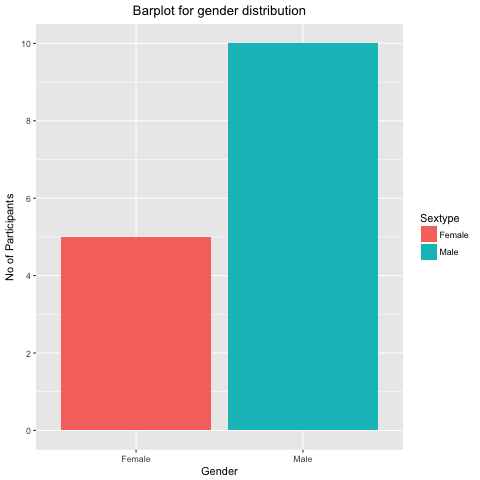
\includegraphics[width=\linewidth]{qc_gender}
	\caption{Barplot of Gender Distribution}
	\end{minipage}
	\hfill
	\begin{minipage}[c]{0.5\linewidth}
	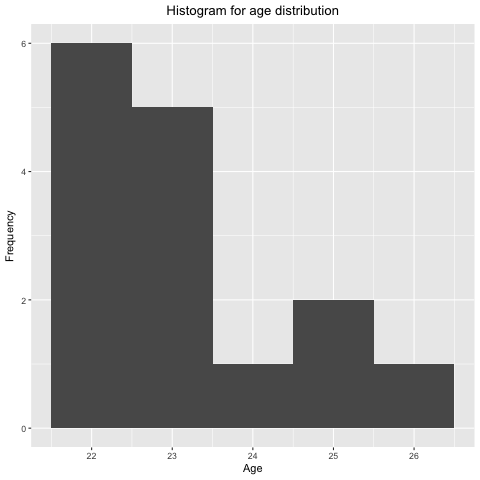
\includegraphics[width=\linewidth]{qc_age}
	\caption{Histogram of age distribution}
	\end{minipage}
\end{figure}

\subsection*{Trait Psychometric Data}
We draw the histogram for Trait Anxiety Inventory(TAI) scores\\
\begin{figure}[!ht]
	\centering
	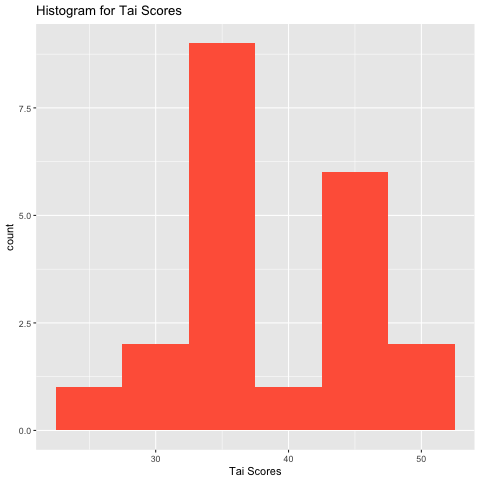
\includegraphics[width=0.8\textwidth]{tai_plot}
	\caption{Histogram of Tai Scores}
	\centering
\end{figure}
\newpage
\subsection*{State Psychometric Data}
For each subject draw the bar plots for all the NASA-TLX subscales per task. This will give two figures per subject per subscale, one for suturing and one for cutting, where the evolution of the scores from the initial to the final session will be evident. \\
\begin{figure}[!ht]
	\begin{minipage}[c]{0.5\linewidth}
	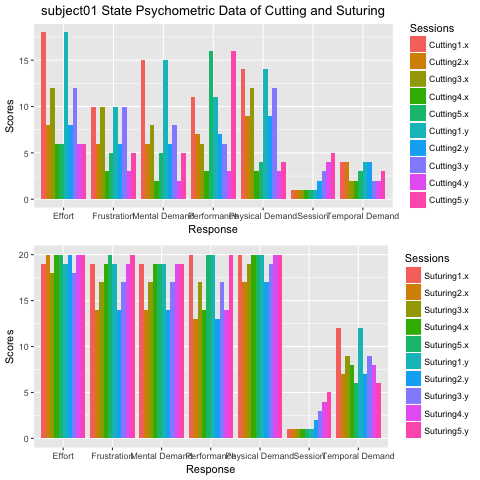
\includegraphics[width=\linewidth]{s1}
	\caption{Subject 1 }
	\end{minipage}
	\hfill
	\begin{minipage}[c]{0.5\linewidth}
	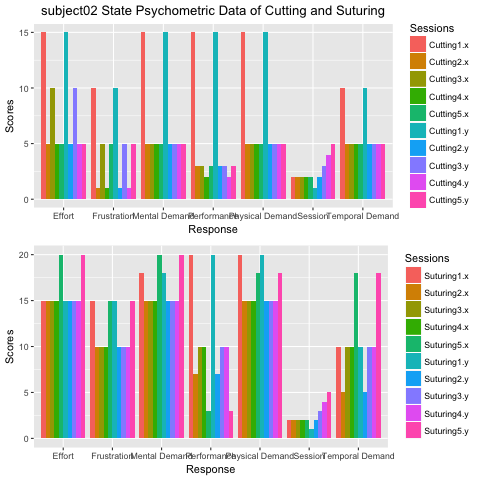
\includegraphics[width=\linewidth]{s2}
	\caption{Subject 2}
	\end{minipage}
\end{figure}
\newpage
\subsection*{Perinasal Perspiration (Stress) Signal Data}
For each session of each subject  we draw the perspiration values using black for baseline, green for cutting, and red for suturing. 
\begin{figure}[!ht]
	\begin{minipage}[c]{0.5\linewidth}
	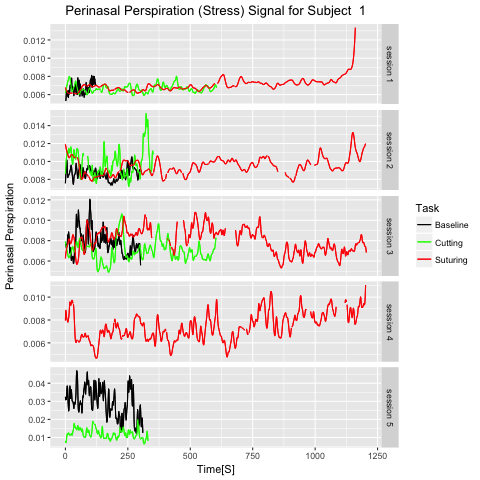
\includegraphics[width=\linewidth]{s1pp}
	\caption{Subject 1 }
	\end{minipage}
	\hfill
	\begin{minipage}[c]{0.5\linewidth}
	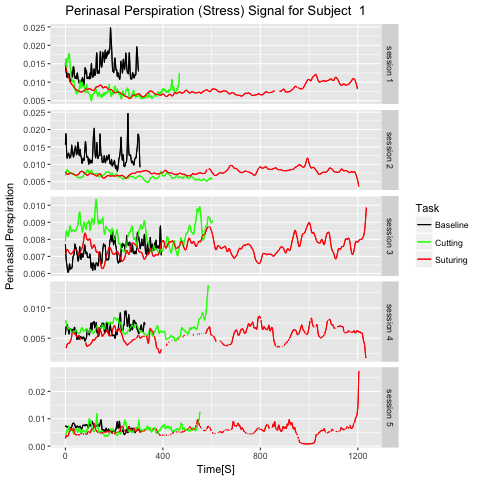
\includegraphics[width=\linewidth]{s2pp}
	\caption{Subject 2}
	\end{minipage}
\end{figure}

\subsection*{Performance Data}
We draw the accuracy and time bar plots of each subject for each session and each task.\\
\begin{figure}[!ht]
	\centering
	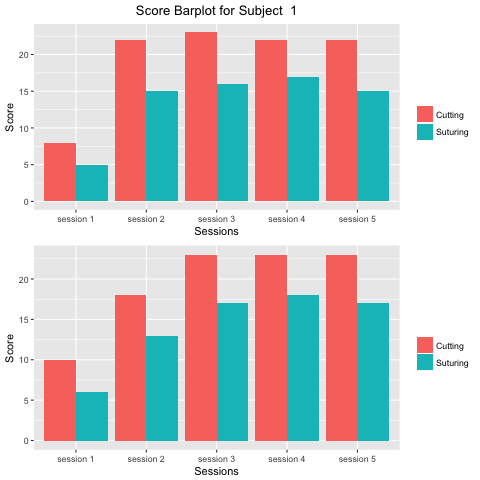
\includegraphics[width=0.8\textwidth]{S1Score_barplot}
	\caption{Subject 1 Score Barplot}
	\centering
\end{figure}
\\
\begin{figure}[!ht]
	\centering
	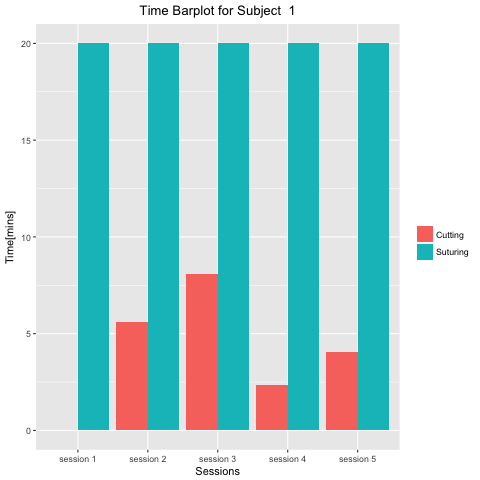
\includegraphics[width=0.8\textwidth]{S1Time_barplot}
	\caption{Subject 1 Time Barplot}
	\centering
\end{figure}\\
\newpage
\section*{Hypothesis Testing}
\addcontentsline{toc}{section}{Hypothesis Testing}

\subsection*{1. Analysis of effect of each attribute on Score}

\textbf{Hypothesis}:\\
$Null Hypothesis : H_0 = $ The score obtained does not depend on the demographics of the subject , session , age , year , sex and perspiration.\\
$Alternate Hypothesis : H_1 = $ The score obtained  depends on the demographics of the subject , session , age , year , sex and perspiration.\\
\\
\textbf{Approach:Linear Modelling}:\\
Linear modeling gives the relationship between the dependent and independent variables. 
In our data set we are finding the hypothesis between each attribute such as Age, sex, year and mean perspiration with the scores of scorer.\\
\begin{figure}[!ht]
	\centering
	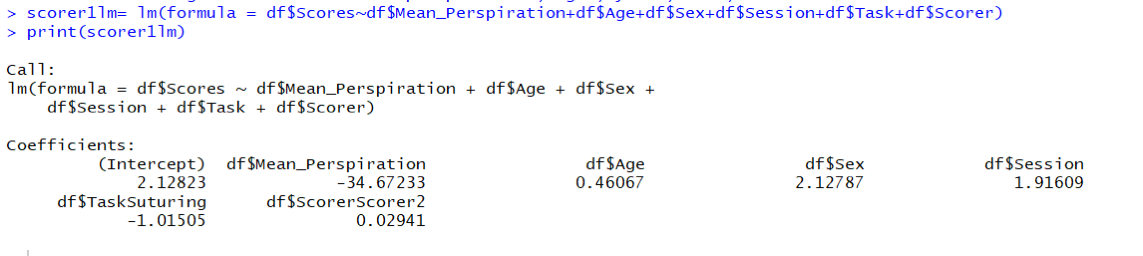
\includegraphics[width=0.8\textwidth]{Picture1}
	\caption{Linear model of score vs all other attributes}
	\centering
\end{figure}
\\
From the above we observe that,\\
Intercept = 2.128 \\
coefficient for mean perspiration = -34.67 \\
coefficient for age = 0.4606\\  
coefficient for sex = 2.127 \\
coefficient for session = 1.916 \\
Based on this, the complete regression equation is \\
Score1=2.128+(-34.67)*meanperspiration+0.4607*Age2.127*Sex+1.916*Session+-1.015*task+0.029*scorer\\
\\
\textbf{Inference}:\\
The above equation informs us that scores will increase by -34.67 for every one percent increase in mean Perspiration value , and score is directly proportional to age which states that the if older age people are hired the score would have increased\\
\\
\subsection*{2. Analysis of Age on Score}

\textbf{Hypothesis}:\\
$Null Hypothesis : H_0 = $ The score obtained does not depend on the age of the subject .\\
$Alternate Hypothesis : H_1 = $ The score obtained depends on the age of the subject .\\
\\
\textbf{Approach:Linear Modelling}:\\
\begin{figure}[!ht]
	\centering
	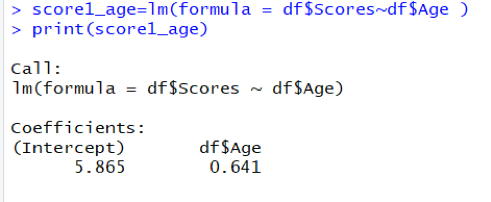
\includegraphics[width=0.8\textwidth]{Picture2}
	\caption{Linear model of score vs age}
	\centering
\end{figure}
\\
From the above we observe that,\\
Intercept = 5.865 \\
coefficient for age = 0.641 \\
Based on this, the complete regression equation is \\
Score= 5.865 + 0.641xAge\\
\\
\textbf{Inference}:\\
The above equation informs us that scores increase with Age.\\

\subsection*{3. Analysis of Year on Score}

\textbf{Hypothesis}:\\
$Null Hypothesis : H_0 = $ The score obtained does not depend on the year of the subject .\\
$Alternate Hypothesis : H_1 = $ The score obtained depends on the year of the subject .\\
\\
\textbf{Approach:Linear Modelling}:\\
\begin{figure}[!ht]
	\centering
	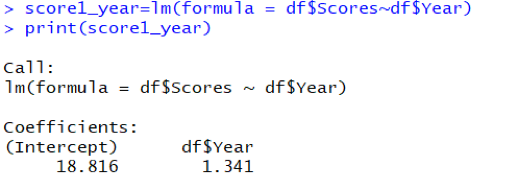
\includegraphics[width=0.8\textwidth]{Picture3}
	\caption{Linear model of score vs year}
	\centering
\end{figure}
\\
From the above we observe that,\\
Intercept = 18.816 \\
coefficient for year = 1.341 \\
Based on this, the complete regression equation is \\
Score= 18.816 + 1.341xYear\\
\\
\textbf{Inference}:\\
The above equation informs us that scores increase with Year . With every 1 year increase, the Score increases with a value of 20.157.\\
\\
\subsection*{4. Analysis of Sex on Score}

\textbf{Hypothesis}:\\
$Null Hypothesis : H_0 = $ The score obtained does not depend on the sex of the subject .\\
$Alternate Hypothesis : H_1 = $ The score obtained depends on the sex of the subject .\\
\\
\textbf{Approach:Linear Modelling}:\\
\begin{figure}[!ht]
	\centering
	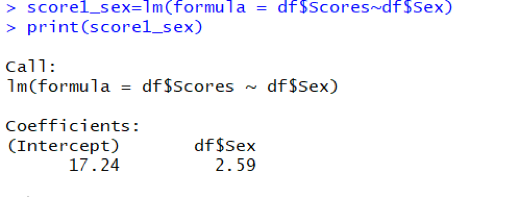
\includegraphics[width=0.8\textwidth]{Picture4}
	\caption{Linear model of score vs sex}
	\centering
\end{figure}
\\
From the above we observe that,\\
Intercept = 17.24 \\
coefficient for sex = 2.59 \\
Based on this, the complete regression equation is \\
Score= 17.24 + 2.59xSex\\
\\
\textbf{Inference}:\\
The above equation informs us that scores depend on sex . \\

\subsection*{5. Analysis of Perspiration on Score}

\textbf{Hypothesis}:\\
$Null Hypothesis : H_0 = $ The score obtained does not depend on the perspiration value  of the subject .\\
$Alternate Hypothesis : H_1 = $ The score obtained depends on the perspiration value of the subject .\\
\\
\textbf{Approach:Linear Modelling}:\\
\begin{figure}[!ht]
	\centering
	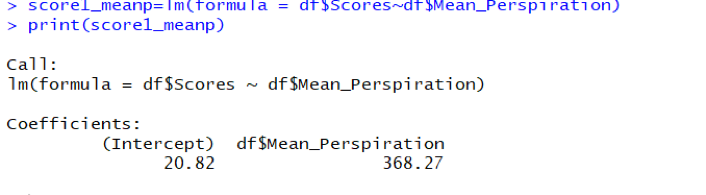
\includegraphics[width=0.8\textwidth]{Picture5}
	\caption{Linear model of score vs Perspiration}
	\centering
\end{figure}
\\
From the above we observe that,\\
Intercept = 20.82 \\
coefficient for perspiration = 368.27 \\
Based on this, the complete regression equation is \\
Score= 20.82 + 368.27xPerspiration\\
\\
\textbf{Inference}:\\
The above equation informs us that scores are directly proportional to the perspiration value. \\


\subsection*{6. Analysis of Scorers on Task:}

\textbf{Hypothesis}:\\
$Null Hypothesis : H_0 = $ The mean of scores is same for both the Scorers\\
$Alternate Hypothesis : H_1 = $ The  mean of scores is different for both the Scorers\\
\\
\textbf{Approach:Wilcox Test}:\\
\begin{figure}[!ht]
	\begin{minipage}[c]{0.5\linewidth}
	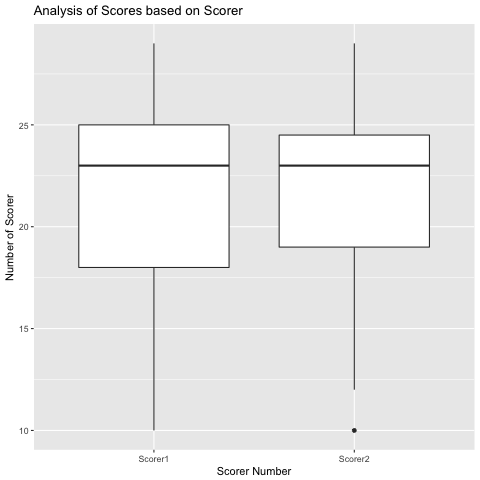
\includegraphics[width=\linewidth]{Cutting_Scores}
	\caption{ Cutting Scores}
	\end{minipage}
	\hfill
	\begin{minipage}[c]{0.5\linewidth}
	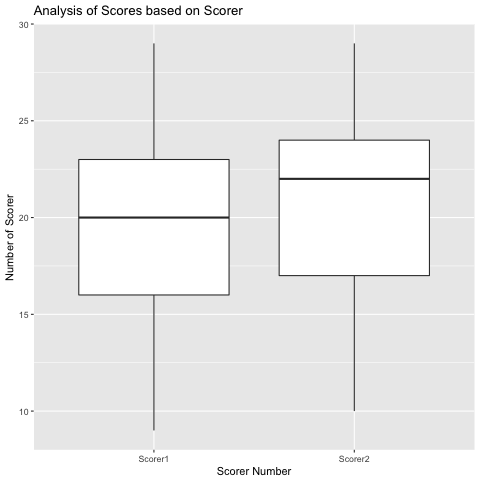
\includegraphics[width=\linewidth]{Suturing_Scores}
	\caption{Suturing Scores}
	\end{minipage}
\end{figure}
\\
Cutting : When performed Wilcox test, p-value is greater than 0.05, which applies the means have not changed\\
Suturing: When performed Wilcox test, p-value is less than 0.05, which states that the means of the scorers is different. \\
\\
\textbf{Inference}:\\
Scorer has an effect for Suturing ,not Cutting\\







\newpage
\section*{Conclusion}
\addcontentsline{toc}{section}{Conclusion}



%-------------------------------------------------------------------------------
% Appendix
%-------------------------------------------------------------------------------
\newpage
\section*{Appendix}
\addcontentsline{toc}{section}{Appendix}
\subsection*{List of Figures}
\addcontentsline{toc}{subsection}{List of Figures}
\subsection*{List of Tables}
\addcontentsline{toc}{subsection}{List of Tables}


%-------------------------------------------------------------------------------
% REFERENCES
%-------------------------------------------------------------------------------
\newpage
\section*{References}
\addcontentsline{toc}{section}{References}




\end{document}

